\chapter{Implementing \textquoteleft Two Degrees of Freedom\textquoteright Controller for First order systems on a
Single Board Heater System}
The aim of this experiment is to implement a 2DOF controller on a
single board heater system.  The target group is anyone who has basic
knowledge of Control Engineering.
\begin{figure}
\centering
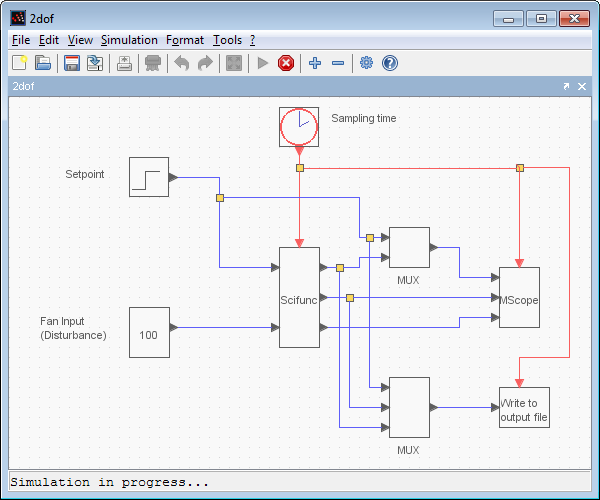
\includegraphics[width=0.9\linewidth]{2-DOF_manual/2dof_xcos.png}
\caption{Xcos interface for this experiment}
\label{Xcos_2dof}
\end{figure}
We have used Scilab with Xcos as an interface for sending and receiving data. This interface is shown in Fig.\ref{Xcos_2dof}. Fan speed and Heater current are the two inputs to the system. For this experiment, the heater current is used as a control effort generated by inputting the various 2-DOF controller parameters like Rc, Sc, Tc and gamma. The fan input could be thought of as an external disturbance.
\section{Theory}
 Degree of freedom as far as the control theory is concerned is the number of parameters on which the plant is no more dependent or the number of parameters that are free to vary. This means that a higher degree of freedom controller makes the plant less susceptible to disturbances. 
Controllers are broadly classified as feedback and feed forward controllers. Feedback controllers are further classified as One Degree of Freedom controller and Two Degree of Freedom controller. Feed forward controllers are those who take the control action before a disturbance disturbs the plant. But this implies an ability to sense the disturbance. Moreover, exact knowledge about the plant is also needed. Nevertheless, due to these restrictions, it is rarely used alone.
A feedback control strategy is as shown in figure \ref{fb}. The reference and the output is continuously compared to generate error which is fed to the controller to take the appropriate control action. Here, exact knowledge about the plant, $G(z)$ and the disturbance, $v$ is not necessary.
\begin{figure}
\begin{center}
\begin{tikzpicture}[auto, node distance=2cm]
\node[input, name=input]{};
\node[sum,right of=input](sum){};
\draw[->](input) -- node{$r$}(sum);
\node[block, right of=sum](gc){$G_c(z)$};
\draw[->](sum)--node{$e$}(gc);
\node[block, right of=gc, node distance=3cm](g){$G(z)$};
\draw[->](gc)--node{$u$}(g);
\node[sum, right of=g,pin={[pinstyle] above:$v$},node distance=2cm](sum2){};
\draw[->](g)--node{}(sum2);
\node[output,right of=sum2,node distance=1cm](output){};
\draw[->](sum2)--node[name=y]{$y$}(output);
\draw [->] (y)--(8.58,-1.5)-|(sum)node[pos=0.88] {$-$};
\end{tikzpicture}
\end{center}
\caption{Feed back control strategy}
\label{fb}
\end{figure}

Solving for y(n), we get
\begin{align}
y(n)&=\frac{G(z)G_c(z)}{1+G(z)G_c(z)}r(n)+\frac 1{1+G(z)G_c(z)}v(n)
\intertext{let,}
T(z)&=\frac{G(z)G_c(z)}{1+G(z)G_c(z)}\\
S(z)&=\frac 1{1+G(z)G_c(z)}
\intertext{this implies}
y(n)&=T(z)r(n)+S(z)v(n)
\intertext{Here it could be seen that the controller has to track the reference input as well as eliminate the effect of external disturbance. But, however from the above equation it could be seen that}
S + T &= 1
\end{align}
Hence it is not possible to achieve both of the requirements, simultaneously in this particular control arrangement. This control arrangement is called {\ttfamily One Degree of Freedom}, abbreviated as 1-DOF.
A {\ttfamily Two Degrees of Freedom} strategy is as shown in figure \ref{2dof}. Here, $G_b$ and $G_f$ together constitute the controller. $G_b$ is in the feedback path and is used to eliminate the effect of disturbances, whereas,$G_f$ is in the feed forward path and is used to help the output track reference input. We need a control law something of the form,
\begin{figure}
\begin{center}
\begin{tikzpicture}[auto,node distance=2cm]
\node[input,name=input](input){};
\node[block,right of=input](gf){$G_f$};
\draw[->](input) -- node{$r$}(gf);
\node[sum,right of=gf,node distance=2cm](sum1){};
\draw[->](gf)--node{}(sum1);
\node[block,right of=sum1](g){$G$};
\draw[->](sum1)--node{$u$}(g);
\node[sum,right of=g,node distance=2cm](sum2){};
\draw[->](g)--node{}(sum2);
\node[output, right of=sum2,node distance=1cm](output){};
\draw[->](sum2)--node[name=y]{$y$}(output){};
\node[block, above of=sum2](h){$H$};
\draw[->](h)--node{$v$}(sum2);
\draw[->](8.015,3.8)--node{$d$}(h);
\node[block, below of=g](gb){$G_b$};
\draw[->](y)|-(gb);
\draw[->](gb)-|node[pos=0.99]{$-$}(sum1);
\end{tikzpicture}
\end{center}
\caption{2DOF Feed back control strategy}
\label{2dof}
\end{figure}

\begin{align}
R_c(z)u(n)&=T_c(z)r(n)-S_c(z)y(n)\label{desired}
\intertext{The terms $R_c$, $S_c$ and $T_c$ are all in polynomials of $z^{-1}$.}
\intertext{It could be seen that,}
G_b &= \frac{S_c}{R_c}
\intertext{and}
G_f &= \frac{T_c}{R_c}\\
\intertext{Consider a plant with model}
A(z)y(n)&=z^{-k}B(z)u(n)+v(n)\label{model}
\intertext{Substituting equation \ref{desired} in equation \ref{model}, we get}
Ay(n)&=z^{-k}\frac{B}{R_c}\bigg[T_cr(n)-S_cy(n)\bigg]+v(n)
\intertext{solving for $y(n)$, we get}
\bigg(\frac{R_cA+z^{-k}BS_c}{R_c}\bigg)y(n)&=z^{-k}\frac{BT_c}{R_c}r(n)+v(n)
\intertext{This can also be written as}
y(n)&=z^{-k}\frac{BT_c}{\phi _{cl}}r(n)+\frac{R_c}{\phi _{cl}}v(n)
\intertext{where}
\phi _{cl}&=R_c(z)A(z)+z^{-k}B(z)S_c(z)
\end{align}
and is known as the closed-loop characteristic polynomial.

Now, we want the following conditions to be satisfied.
\begin{enumerate}
\item The zeros of $\phi _{cl}$ should be inside the unit circle, so that the closed-loop system becomes stable. 
\item The value of $z^{-k}\frac{BT_c}{\phi _{cl}}$ must be close to unity so that reference tracking is achieved 
\item The value of $\frac{R_c}{\phi _{cl}}$ must be as small as possible to achieve disturbance rejection
\end{enumerate}
We would now see the pole placement controller approach to design a 2DOF controller.\cite{kmmdc09}

\section{Designing 2-DOF controller using pole placement control approach}
A 2DOF pole placement controller is as shown in the figure \ref{2dofppc}
\begin{figure}
\begin{center}
\begin{tikzpicture}[auto,node distance=2cm]
\node[input](input){};
\node[block,right of=input](tcbyrc){$\gamma \frac{T_c(z)}{R_c(z)}$};
\draw[->](input)--node{$r$}(tcbyrc);
\node[sum,right of=tcbyrc,node distance=2cm](sum1){};
\draw[->](tcbyrc)--node{}(sum1);
\node[block,right of=sum1](plant){$G=z^{-k}\frac{B(z)}{A(z)}$};
\draw[->](sum1)--node{$u$}(plant);
\node[output,right of=plant](output){};
\draw[->](plant)--node[name=y]{$y$}(output);
\node[block,below of=plant](scbyrc){$\frac{S_c}{R_c}$};
\draw[->](y)|-node{}(scbyrc);
\draw[->](scbyrc)-|node[pos=0.99]{$-$}(sum1);
\end{tikzpicture}
\end{center}
\caption{2-DOF pole placement controller}
\label{2dofppc}
\end{figure}

It should be noted that the effect of external disturbance will not be considered for this section.
We want the closed loop transfer function to behave in such a way so that the output $y$ is related to the setpoint $r$ in the following manner
\begin{align}
Y_m(z)&=\gamma z^{-k}\frac{B_r}{\phi_{cl}}R(z)\label{modeloutput}
\intertext{Here, $Y_m(z)$ means the model output. $\phi_{cl}$ is nothing but the closed loop characteristic polynomial obtained by the desired location analysis.}
\intertext{The value of gamma is chosen in such a way so that at steady-state the output of the model is equal to the setpoint.}
\gamma&=\frac{\phi_{cl(1)}}{B_r(1)}
\intertext{Simplifying the block diagram shown in figure \ref{2dofppc} yields}
Y&=\gamma z^{-k}\frac{BT_c}{AR_c+z^{-k}BS_c}R\label{blkdigoutput}
\intertext{Here we have dropped the argument of $z$ for convenience}
\intertext{On comparing equation \ref{modeloutput} and \ref{blkdigoutput} we can see that}
\frac{BT_c}{AR_c+z^{-k}BS_c}&=\frac{B_r}{\phi_{cl}}\label{comparison}
\intertext{Here after factorization of the LHS we can expect some cancellations between the numerator and the denominator  thereby making the $deg B_r < deg B$. But the cancellations ,if any, must be between $stable$ poles and zeros. One should avoid the cancellation of an unstable pole with a zero.}
\intertext{Hence, we differentiate the factors as $good$ and $bad$ factors. Therefore we write $A$ and $B$ as }
A&=A^gA^b\\
B&=B^gB^b
\intertext{We also split $R_c,S_c$ and $T_c$ as shown}
R_c&=B^gR_1\\
S_c&=A^gS_1\\
T_c&=A^gT_1
\intertext{Hence, the equation \ref{comparison} becomes}
\frac{B^gB^bA^gT_1}{A^gA^bB^gR_1+z^{-k}B^gB^bA^gS_1}&=\frac{B_r}{\phi_{cl}}
\intertext{After appropriate cancellations, we obtain}
\frac{B^bT_1}{A^bR_1+z^{-k}B^bS_1}&=\frac{B_r}{\phi_{cl}}\label{aftercancelation}
\intertext{Equating the LHS and RHS of equation \ref{aftercancelation} we obtain}
B^bT_1&=B_r\label{Br}\\
A^bR_1+z^{-k}B^bS_1&=\phi_{cl}\label{aryabhatta}
\intertext{Equation \ref{aryabhatta} is known as the aryabhatta's identity and can be used to solve for $R_1$ and $S_1$. There are many options to choose for the value of $T_1$. By choosing $T_1$ to be equal to $S_1$ the 2-DOF controller is reduced to 1-DOF controller. We usually choose $T_1$=1.}
\intertext{Equation \ref{Br} becomes}
B^b&=B_r
\intertext{hence the expression of gamma is now changed to}
\gamma&=\frac{\phi_{cl(1)}}{B^b(1)}
\intertext{and the desired closed loop transfer function now becomes}
Y_m(z)&=\gamma z^{-k}\frac{B^b}{\phi_{cl}}R(z)
\end{align}
This implies that the open loop model imposes two limitations on the closed loop model.
\begin{itemize}
\item The bad portion of the open loop model cannot be canceled out and it appears in the closed loop model. 
\item The open loop plant delay cannot be removed or minimized,i.e. the closed loop model cannot be made faster then the open loop model.  
\end{itemize}
\section{Step by step procedure to design and implement a 2-DOF controller}
We obtain a first order transfer function of the plant using the step test approach.The model so obtained is
\begin{align}
G(s)&=\frac{0.42}{35.61s+1}
\intertext{with time constant $\tau = 35.6 sec$ and gain $K=0.42$}
\intertext{After discretization with sampling time = 1 second, we obtain}
G(z)&=\frac{0.0116304}{z-0.9723086}\\
&=\frac{0.0116304z^{-1}}{1-0.9723086z^{-1}}
\end{align}
%Discretization can be done using the scilab code {\ttfamily c2d.sce}.
We would now define good and bad terms
\begin{align*}
A^g&=1-0.9723086z^{-1}\\
A^b&=1\\
B^{g}&=0.0116304\\
B^{b}&=1
\intertext{Let us now define the transient specifications. We choose,}
\text{Rise time} &=100 \text{ seconds}
\intertext{No. of samples per rise time ($N_r$) is calculated as}
N_r&\le\frac{\text{Rise time}}{\text{Sampling time}}\\
&=100
\intertext{next}
\omega&=\frac{\pi}{2N_r}\\
&=0.015708
\intertext{We choose,}
Overshoot(\epsilon)&=0.05.........i.e 5\%\\
\rho&\le \epsilon ^{\omega / \pi}\\
&=0.860
\intertext{Let us now calculate 2DOF Controller parameters.
The closed loop characteristic polynomial is given by}
\phi _{cl}&= 1-z^{-1}2\rho cos\omega + \rho ^2z^{-2}\\
&=1-1.7198065z^{-1}+0.7396z^{-2}
\intertext{But according to equation \ref{aryabhatta}}
A^bR_1+z^{-k}B^bS_1&=\phi_{cl}
\intertext{Recall that we had not considered external disturbance in the block diagram shown in figure\ref{2dofppc}. However, we can still, up to some extent, take care of the disturbances. This is achieved by using the internal model principle. If a model of step is present inside the loop, step disturbances can be rejected. We can apply this by forcing $R_c$ to have this term. A step model is given by}
1(z)&=\frac{1}{1-z^{-1}}
\intertext{Let the denominator of the step model be denoted as $\Delta$}
\Delta &= 1-z^{-1}
\intertext{Therefore,}
R_c&=B^g\Delta R_1
\intertext{$\Delta$ has a root which lies on the unit circle. Hence it has to be treated as a bad part and should not be canceled out. Hence, we should make sure that all of the occurrences of $R_1$ have this term.}
\end{align*}
Therefore,
\begin{align}
\phi_{cl}&=A^b\Delta R_1+z^{-k}B^bS_1
\end{align}
Hence,
\begin{align*}
A^b\Delta R_1+z^{-k}B^bS_1&=1-1.7198065z^{-1}+0.7396z^{-2}
\end{align*}
The expression is known as the Aryabhatta Identity and is solved using rigorous Matrix calculations. The explanation of this operation is not considered here. You may refer to the book "Digital Control" by Prof. Kannan Moudgalya \cite{kmmdc09} 
%\intertext{The expression, however, does not satisfy the conditions required for solving the Aryabhatta Identity.} 
%\intertext{Let,}
%\begin{align*}
%R_1&=1-0.7396z^{-1}
%\intertext{therefore}
%S_1&=0.0198\\
%R_c&=B^g\Delta R_1
%\intertext{therefore}
%R_c&=0.0116304-0.0229175z^{-1}+0.0112871z^{-2}\\
%S_c&=A^gS_1
%\intertext{hence}
%S_c&=0.0004641-0.0004512z^{-1}\\
%T_c&=A^gT_1
%\intertext{therefore}
%T_c&=1-0.9723z^{-1}\\
%\gamma&=\frac{\phi_{cl(1)}}{B^b(1)}\\
%&=0.0004641
%\intertext{$\phi_{cl(1)}$ means for $z=1$, steady-state. So, we get}
\begin{align*}
R_c&=R_{c1}+R_{c2}z^{-1}+R_{c3}z^{-2}\\
&=0.0116304-0.0229175z^{-1}+0.0112871z^{-2}\\
S_c&=S_{c1}+S_{c2}z^{-1}\\
&=0.0004641-0.0004512z^{-1}\\
T_c&=T_{c1}+T_{c2}z^{-1}\\
&=1-0.9723z^{-1}\\
\gamma&=0.0004641
\end{align*}

Scilab code {\ttfamily twodof\_para.sce} does these calculations.  This code utilizes various other scilab codes provided at the end of this document. Execute this scilab code with the first order transfer function for your SBHS. You would obtain a Z-Transformed transfer function for the continuous time transfer function you input. You would also obtain the various parameters of 2dof controller as shown in figure \ref{2-DOF_para}
\begin{figure}
\centering
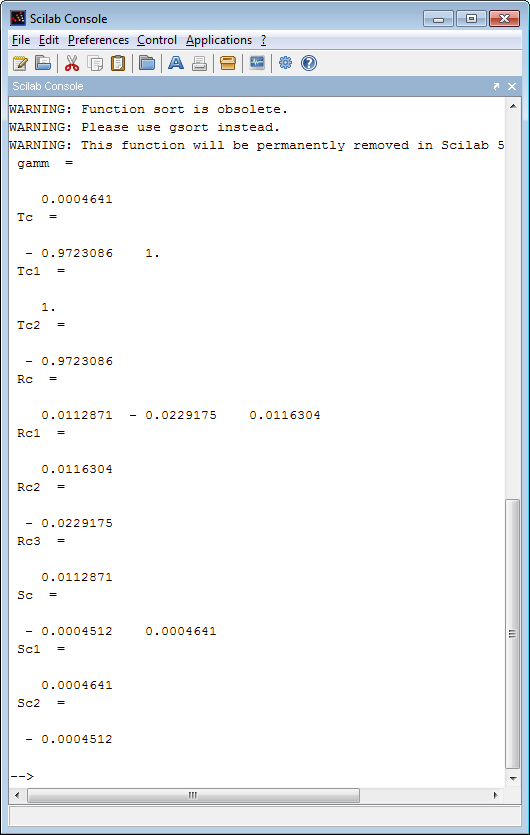
\includegraphics[width=0.8\linewidth]{2-DOF_manual/2dof_console}
\caption{Scilab output for \ttfamily 2DOF\_para.sce}
\label{2-DOF_para}
\end{figure}
\footnote{ NOTE:- The scilab codes are given at the end of this document.}
After execution of {\ttfamily twodof\_para.sce}, run the Xcos code {\ttfamily twodof.xcos} with required setpoint value and observe the temperature profile. The performance of the controller is shown in figure \ref{rt_127}Make sure that you input the sampling time(Clock period) same as the one you used for discretization of the continuous time plant transfer function.
\begin{figure}
\centering
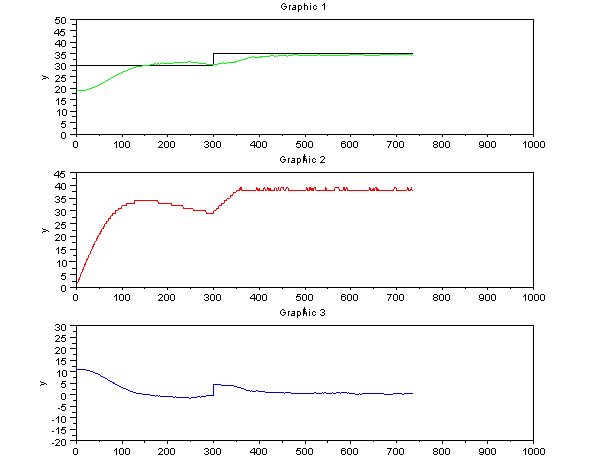
\includegraphics[width=\linewidth]{2-DOF_manual/2dof_resp.png}
\caption{Implementation of 2DOF controller}
\label{rt_127}
\end{figure}
It could be seen that the output (temperature) tracks the setpoint irrespective of the step changes in the fan speed.
We can see that the Over shoot turns out to be 6\% and rise time turns out to be 60 seconds, which is acceptable.

 To implement a second order transfer function, input the correct second order transfer function in {\tt twodof\_para.sce}. Also, make sure you comment the first order control law equation and uncomment the second order control law equation in {\tt twodof.sci} file.

\subsection{Implementing 2dof controller on SBHS, virtually}
The step by step procedure for conducting an experiment virtually is explained in section \ref{vlabsexpt}. The required .sce file is twodof.sce. You will find this file in the {\tt 2dof\_controller} directory under virtual folder. The necessary code is listed in the section \ref{2dofcode}


\section{Scilab Code}\label{2dofcode}
\begin{code}
  \ccaption{c2d.sce}{\ttfamily c2d.sce}
\lstinputlisting{2-DOF_manual/2dof/c2d.sce}
\end{code}
\begin{code}
\ccaption{2-DOF\_para.sce}{\ttfamily 2-DOF\_para.sce}
\lstinputlisting{2-DOF_manual/2dof/2-DOF_para.sce}
\end{code}
\begin{code}
  \ccaption{2dof.sci }{\ttfamily 2dof.sci}
\lstinputlisting{2-DOF_manual/2dof/2dof.sci}
\end{code}
\begin{code}
  \ccaption{cindep.sci}{\ttfamily cindep.sci}
\lstinputlisting{2-DOF_manual/2dof/cindep.sci}
\end{code}
\begin{code}
  \ccaption{clcoef.sci}{\ttfamily clcoef.sci}
\lstinputlisting{2-DOF_manual/2dof/clcoef.sci}
\end{code}
\begin{code}
 \ccaption{clcoef.sci}{\ttfamily clcoef.sci}
\lstinputlisting{2-DOF_manual/2dof/clcoef.sci}
\end{code}
\begin{code}
  \ccaption{cosfil\_ip.sci}{\ttfamily cosfil\_ip.sci}
\lstinputlisting{2-DOF_manual/2dof/cosfil_ip.sci}
\end{code}
\begin{code}
  \ccaption{desired.sci}{\ttfamily desired.sci}
\lstinputlisting{2-DOF_manual/2dof/desired.sci}
\end{code}
\begin{code}
  \ccaption{indep.sci}{\ttfamily indep.sci}
\lstinputlisting{2-DOF_manual/2dof/indep.sci}
\end{code}
\begin{code}
  \ccaption{left\_prm.sci}{\ttfamily left\_prm.sci}
\lstinputlisting{2-DOF_manual/2dof/left_prm.sci}
\end{code}
\begin{code}
  \ccaption{makezero.sci}{\ttfamily makezero.sci}
\lstinputlisting{2-DOF_manual/2dof/makezero.sci}
\end{code}
\begin{code}
 \ccaption{move\_sci.sci}{\ttfamily move\_sci.sci}
\lstinputlisting{2-DOF_manual/2dof/move_sci.sci}
\end{code}
\begin{code}
 \ccaption{polmul.sci}{\ttfamily polmul.sci}
\lstinputlisting{2-DOF_manual/2dof/polmul.sci}
\end{code}
\begin{code}
 \ccaption{polsize.sci}{\ttfamily polsize.sci}
\lstinputlisting{2-DOF_manual/2dof/polsize.sci}
\end{code}
\begin{code}
  \ccaption{polsplit3.sci}{\ttfamily polsplit3.sci}
\lstinputlisting{2-DOF_manual/2dof/polsplit3.sci}
\end{code}
\begin{code}
  \ccaption{polyno.sci}{\ttfamily polyno.sci}
\lstinputlisting{2-DOF_manual/2dof/polyno.sci}
\end{code}
\begin{code}
 \ccaption{pp\_im.sci}{\ttfamily pp\_im.sci}
\lstinputlisting{2-DOF_manual/2dof/pp_im.sci}
\end{code}
\begin{code}
  \ccaption{rowjoin.sci}{\ttfamily rowjoin.sci}
\lstinputlisting{2-DOF_manual/2dof/rowjoin.sci}
\end{code}
\begin{code}
  \ccaption{seshft.sci}{\ttfamily seshft.sci}
\lstinputlisting{2-DOF_manual/2dof/seshft.sci}
\end{code}
\begin{code}
  \ccaption{t1calc.sci}{\ttfamily t1calc.sci}
\lstinputlisting{2-DOF_manual/2dof/t1calc.sci}
\end{code}
\begin{code}
 \ccaption{xdync.sci}{\ttfamily xdync.sci}
\lstinputlisting{2-DOF_manual/2dof/xdync.sci}
\end{code}
\begin{code}
 \ccaption{zpowk.sci}{\ttfamily zpowk.sci}
\lstinputlisting{2-DOF_manual/2dof/zpowk.sci}
\end{code}
%\bibliography{2-DOF}

